\documentclass[a4paper]{article}
\usepackage[english]{babel}
\usepackage[utf8x]{inputenc}
\usepackage[T1]{fontenc}
\usepackage[left=3.0cm, right=2.0cm, top=2.5cm, bottom=2.5cm]{geometry}
\usepackage{amsmath}
\usepackage{graphicx}
\usepackage{caption}
\usepackage{float}

\date{}

\begin{document}
\newpage
\thispagestyle{empty}


\begin{center}
\centering

\includegraphics[keepaspectratio,scale=2]{WUT_logo.jpeg} \\[1.0cm]
{\fontsize{17}{17}\selectfont
\textsc{Warsaw University of Technology \\[1.5cm]
Faculty of Power and Aeronautical Engineering  \\[.5cm]
Institute of Heat Engineering  \\[1.0cm]}
\huge{Aerospace Engineering \\[1.7cm]}}
\fontsize{30}{30}\selectfont
\textbf{Detonation parameters of ethane-oxygen  mixture \\[3.0cm]}
\huge{Agata Łuczak \\ 271302}
\end{center}


\newpage


\begin{abstract}
    The purpose of this project was an analysis of the role and the impact of initial temperature, pressure and equivalence ratio in a process of ethane-oxygen mixture's Chapman-Jouguet detonation. The simulation was set up using Cantera and SDToolbox in Python and the results of performed calculations were saved in a data file, but also depicted as plots.
\end{abstract}
\section{Introduction and mathematical model}
Detonation is a rapid and violent combustion. It involves a supersonic exothermic front accelerating through a medium that eventually drives a shock front propagating directly in front of it. Detonation can happen in solid and liquid explosives as well as in reactive gases.\\
The Shock \& Detonation Toolbox used in the simulation is an open-source software library that enables the solution of standard problems for gas-phase explosions using realistic thermochemistry and detailed chemical kinetics. SDToolbox includes numerical routines for the computation of CJ detonation speed and post-detonation state.The Chapman-Jouguet solution is often used to approximate the properties of an ideal steady detonation wave. In particular, detonation waves are often observed to propagate at speeds within 5-10\% of their theoretical CJ speeds in experimental situations where the waves are far from failure.\\
Ethane-oxygen mixture's detonation simulation was conducted under specific conditions, for $20$ various temperatures, pressures, equivalence ratios. As results parameters such as: CJ detonation velocity,pressure,density and temperature were acquired.\\\\
\subsection{Stoichiometry}
\begin{center}
    $2C_2H_6 +7O_2=4CO_2+6H_2O$\\
    \bigskip
   (F/A)$_{stoichiometric}$ = \( \frac{2}{7} \) = $0,285714$\\
   \bigskip
   $\phi =  \frac{F/A}{(F/A)_{stoichiometric}}$\\
   \bigskip
   F/A = $\phi*(F/A)_{stoichiometric}$\\
   \bigskip
   A = $\frac{F}{\phi*(F/A)_{stoichiometric}}$
\end{center}
Assuming constant number of ethane moles, only the number of oxygen moles would change accordingly to the equation above.     
\subsection{Boundary conditions}
The written program itself allows to input any values of the fundamental parameters, however, this specific simulation was conducted for: 
\begin{center}
    $P_{min} = 101325 Pa$\\
    \bigskip
    $P_{max} = 405300 Pa$\\
    \bigskip
    $T_{min} = 290 K$\\
    \bigskip
    $T_{max}= 850 K$\\
    \bigskip
    $\phi_{min} = 0.1$\\
    \bigskip
    $\phi_{max} = 2$\\
\end{center}
\newpage
\section{Results}
Acquired through simulation data was successfully imported to .csv files and plots are shown below.
\subsection{CJ detonation velocity}
\begin{figure}[H]
\centering
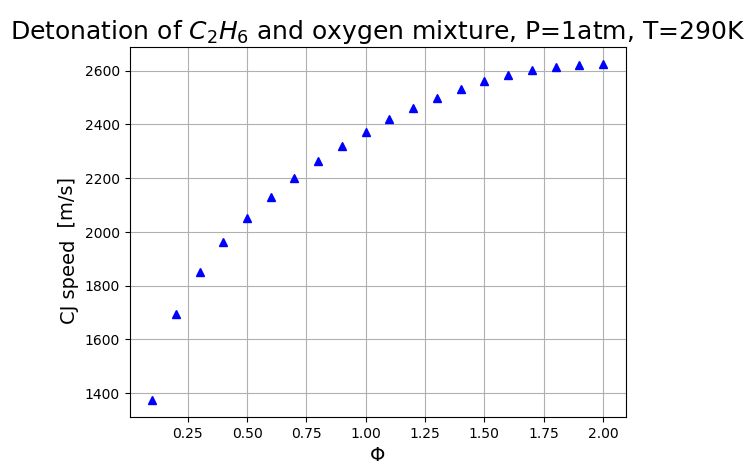
\includegraphics[width=0.8\textwidth]{CJspeed_Fi.png}
\caption{Detonation velocity as a function of equivalence ratio}
\end{figure}

\begin{figure}[H]
\centering
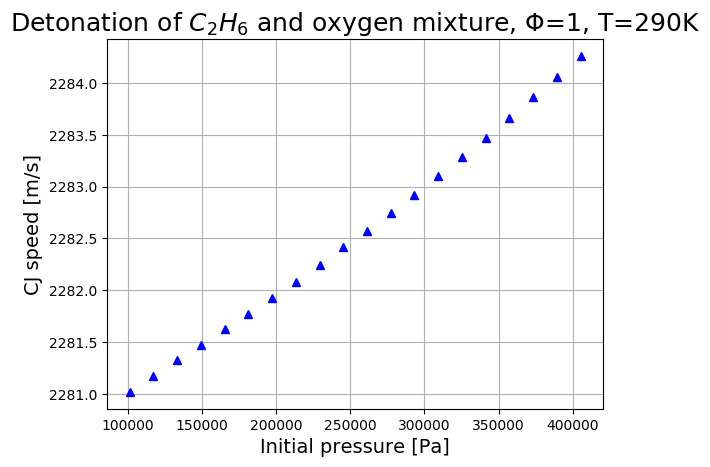
\includegraphics[width=0.8\textwidth]{CJspeed_Pi.png}
\caption{Detonation velocity as a function of initial pressure}
\end{figure}

\begin{figure}[H]
\centering
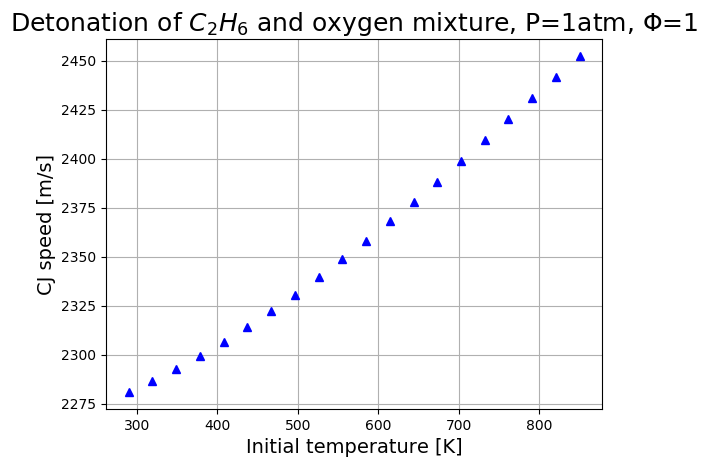
\includegraphics[width=0.8\textwidth]{CJspeed_Ti.png}
\caption{Detonation velocity as a function of initial temperature}
\end{figure}

CJ detonation velocity increases with increasing pressure, temperature and $\phi$. Velocity doesn't rise as fast even after significantly increasing initial pressure. It seems that in conducted simulation $\phi$ has the biggest influence on the velocity, since the growth of CJ speed is the most noticeable for such range of equivalence ratio. Functions of initial temperature and pressure appear to be almost linear.

\subsection{CJ detonation density}
\begin{figure}[H]
\centering
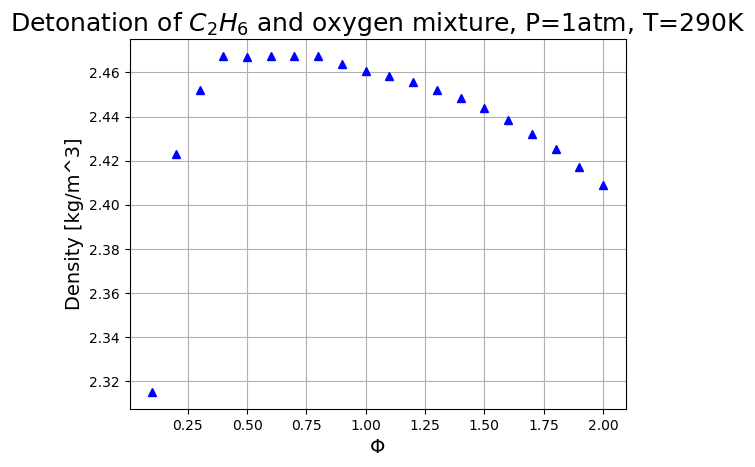
\includegraphics[width=0.8\textwidth]{density_Fi.png}
\caption{Detonation density as s function of equivalence ratio}
\end{figure}

\begin{figure}[H]
\centering
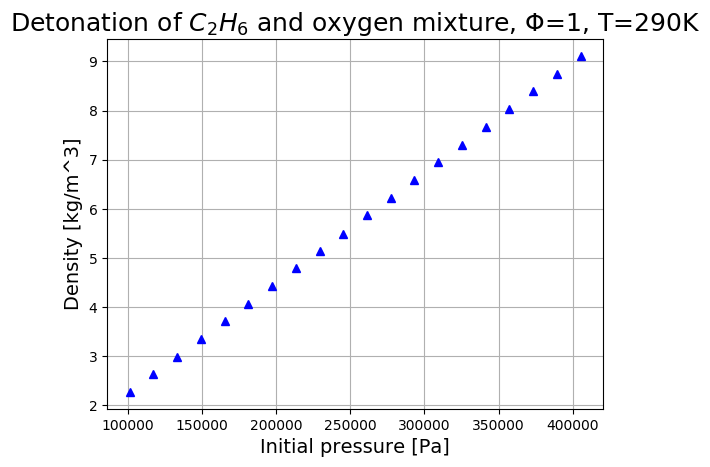
\includegraphics[width=0.8\textwidth]{density_Pi.png}
\caption{Detonation density as s function of initial pressure}
\end{figure}

\begin{figure}[H]
\centering
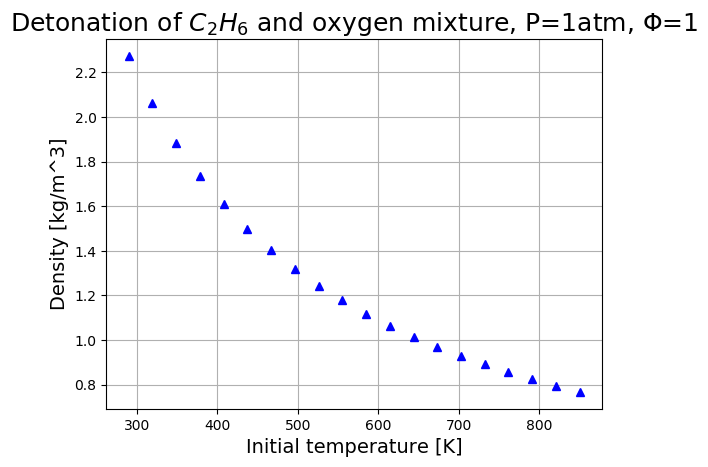
\includegraphics[width=0.8\textwidth]{density_Ti.png}
\caption{Detonation density as s function of initial temperature}
\end{figure}

CJ detonation density increases very rapidly, although, very small amounts for lower values of $\phi$ and around 0.5 starts to decrease. When it comes to initial pressure's influence on density, its value grows quite linearly with the growth of the pressure. Quadrupling pressure causes similar increase of density's value. For initial temperature, however, density plummets drastically from around 2.2 \( \frac{kg}{m^{3}} \) to around 0.8 \( \frac{kg}{m^{3}} \).

\subsection{CJ detonation pressure}
\begin{figure}[H]
\centering
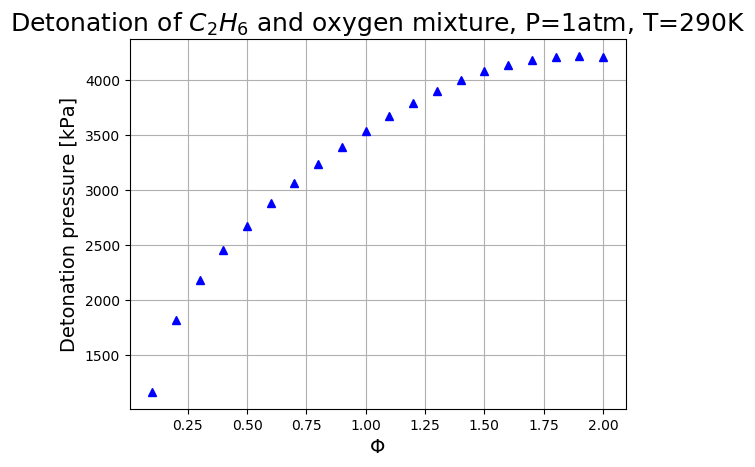
\includegraphics[width=0.8\textwidth]{pressure_Fi.png}
\caption{Detonation pressure as s function of equivalence ratio}
\end{figure}

\begin{figure}[H]
\centering
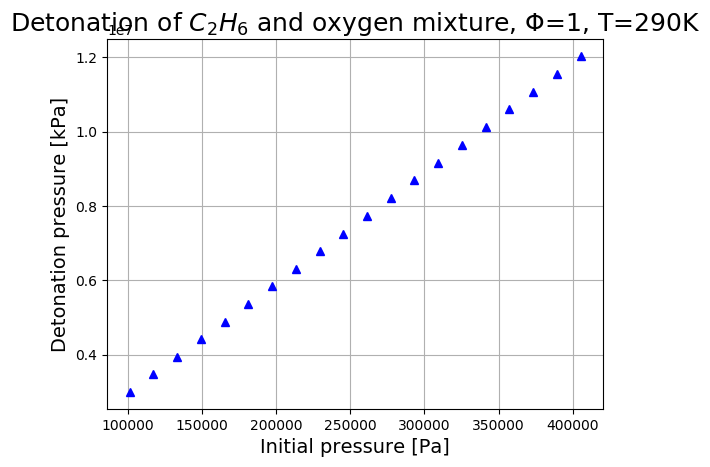
\includegraphics[width=0.8\textwidth]{pressure_Pi.png}
\caption{Detonation pressure as s function of initial pressure}
\end{figure}

\begin{figure}[H]
\centering
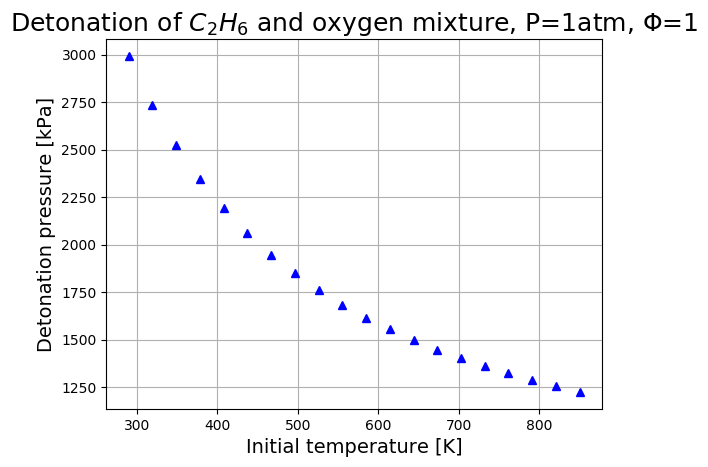
\includegraphics[width=0.8\textwidth]{pressure_Ti.png}
\caption{Detonation pressure as s function of initial temperature}
\end{figure}

CJ detonation pressure increases exponentially as a function of $\phi$, increases linearly with the growth of initial pressure and decreases also exponentially for higher values of initial temperatures. It's worth noting how great are the values of detonation pressure as a function of initial pressure, they go from around 3000 MPa to 12000 MPa.

\subsection{CJ detonation temperature}
\begin{figure}[H]
\centering
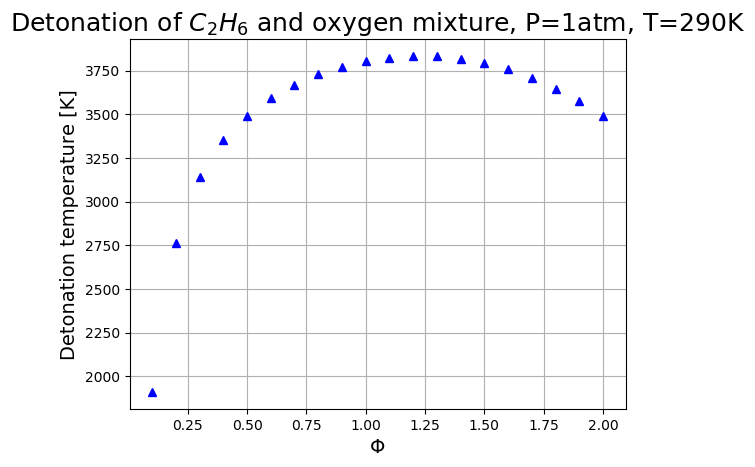
\includegraphics[width=0.8\textwidth]{temperature_Fi.png}
\caption{Detonation temperature as a function of equivalence ratio}
\end{figure}

\begin{figure}[H]
\centering
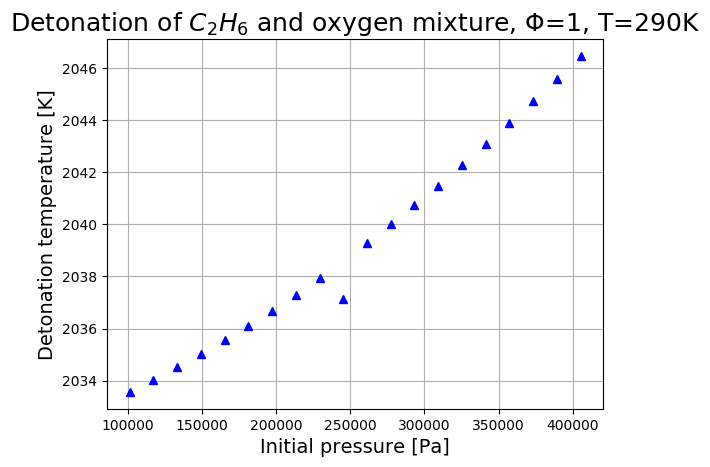
\includegraphics[width=0.8\textwidth]{temperature_Pi.png}
\caption{Detonation temperature as a function of initial pressure}
\end{figure}

\begin{figure}[H]
\centering
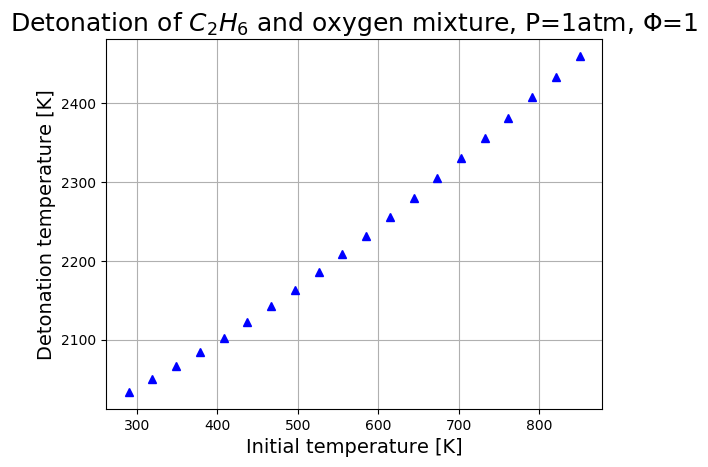
\includegraphics[width=0.8\textwidth]{temperature_Ti.png}
\caption{Detonation temperature as a function of initial temperature}
\end{figure}

CJ detonation temperature as a function of $\phi$ has an exponential character, for lower ratios the value increases and then for higher goes down. In the plot for various initial pressures there's one abnormal point around 250 kPa, however, for the rest of simulation points it's an increasing function. As initial temperature rises so does the detonation temperature, but they reach much higher values, which isn't a surprise.

\section{Conclusion}
Conducted study proves that detonation of ethane-oxygen mixture is highly dependant on fundamental parameters such as temperature, pressure and $\phi$.\\

\begin{thebibliography}{9}
\bibitem{1}
\texttt{http://shepherd.caltech.edu/EDL/PublicResources/sdt/doc/QuickReferenceSDT.pdf}
\bibitem{2} 
\texttt{https://www.sciencedirect.com/topics/engineering/detonations}
\bibitem{3}
\texttt{https://github.com/MortenTabaka/Calculating-detonation-parameters-of-propane-oxygen-mixture/blob/master/Code.txt}
\end{thebibliography}

\end{document}